%% Q1
Each letter moves \textbf{two places forward}: T$\rightarrow$V, E$\rightarrow$G, A$\rightarrow$C, M$\rightarrow$O.
LIFE $\rightarrow$ L$+2=$N, I$+2=$K, F$+2=$H, E$+2=$G, giving \textbf{NKHG}.

%% Q2 fig
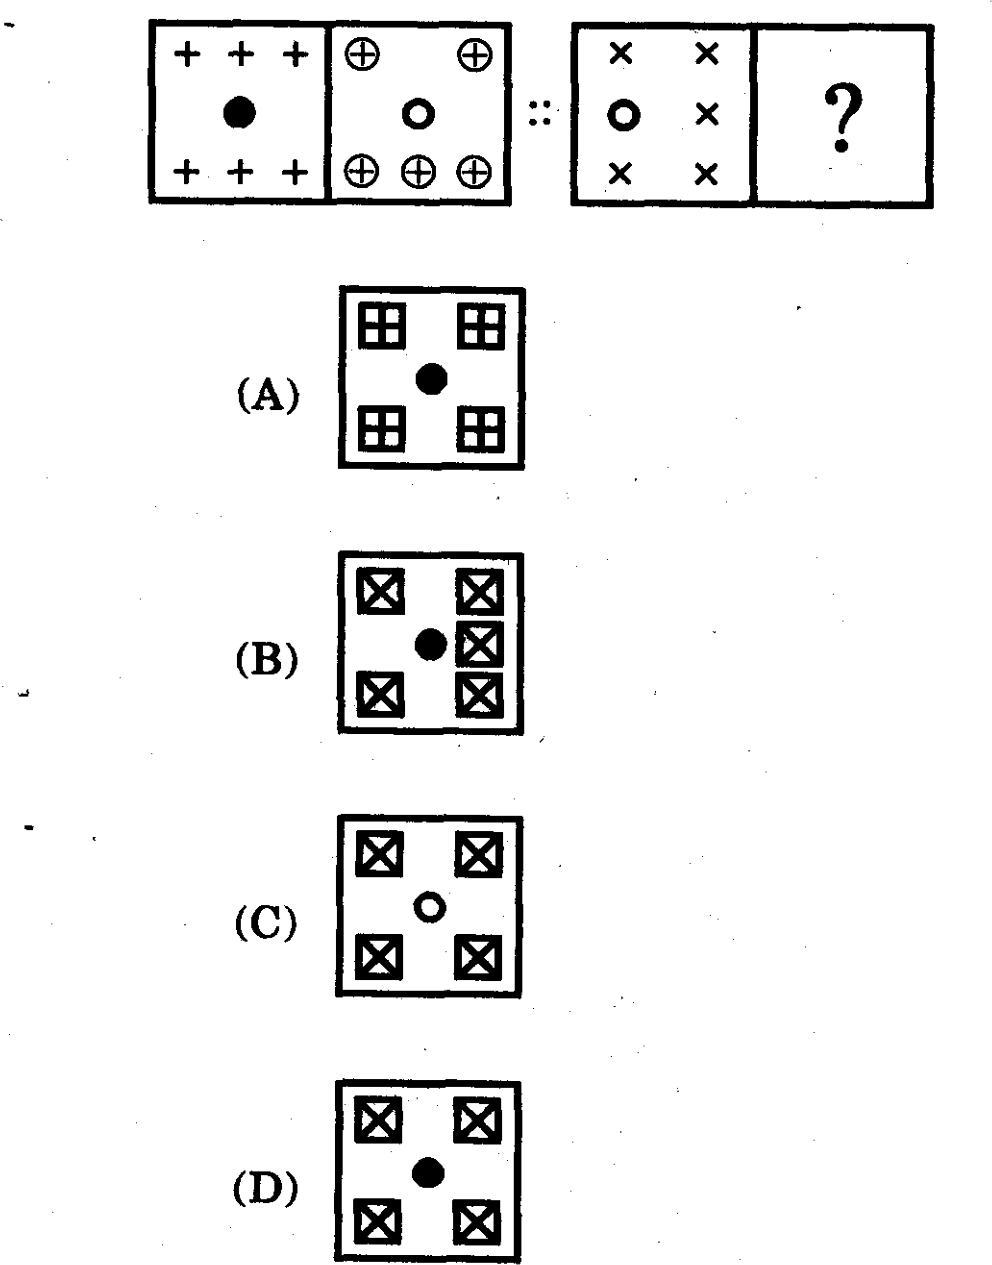
\includegraphics[height=6.2cm]{fig/dec08_q2.png}

%% Q2 opts
Figure (A)
Figure (B)
Figure (C)
Figure (D)

%% Q2
From the first figure to the second, three things happen. Each symbol is \textbf{enclosed} ($+\rightarrow\oplus$), the number of symbols \textbf{falls by one} ($6\rightarrow5$), and the central dot \textbf{changes shade} (filled $\rightarrow$ hollow).
Apply the same to the third figure: $\times\rightarrow\boxtimes$, $5\rightarrow4$ symbols, and the hollow dot becomes \textbf{filled}. Figure \textbf{(D)} fits.
\why{(A) uses boxed plus signs; (B) has five symbols; (C) keeps the dot hollow.}

%% Q3
Look for the pattern ``8 7 x'' where x $\neq 3$:
\begin{center}\ttfamily 8 9 8 \textbf{7} 6 2 2 6 3 2 6 9 7 3 2 8 \textbf{7} 2 7 7 8 7 3 7 7 9 4\end{center}
``8 7 6'' (position 3--5) and ``8 7 2'' qualify, while ``8 7 3'' is excluded. Count $=\mathbf{2}$.

%% Q4
Nitin says 32, 31, 30, \ldots; Shashank says 1, 3, 5, \ldots. At the $n$-th count Nitin says $33-n$ and Shashank says $2n-1$.
$33-n=2n-1\Rightarrow n=34/3$, which is not a whole number, so they \textbf{never say the same number together}: none of the above.

%% Q5
Decode (C): $18\div3-6+8+4=12$, i.e.\ $6-6+8+4=12$ \checkmark.
Check the others: (A) $18\div3=6$ but the right side $8\div4-12$ is not 6; (B) $18>13+128-48$ is false; (D) $18>18+8-4+12=34$ is false.

%% Q6 fig
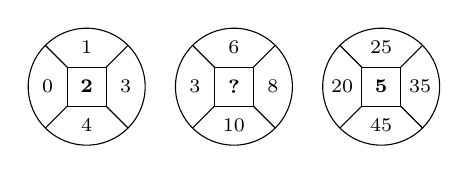
\begin{tikzpicture}[scale=0.55,font=\scriptsize]
\foreach \cx/\t/\l/\r/\b/\c in {0/1/0/3/4/2, 3.4/6/3/8/10/?, 6.8/25/20/35/45/5}{
 \draw (\cx,0) circle(1.35); \draw (\cx-0.45,-0.45) rectangle (\cx+0.45,0.45);
 \draw (\cx-0.45,0.45)--(\cx-0.95,0.95); \draw (\cx+0.45,0.45)--(\cx+0.95,0.95);
 \draw (\cx-0.45,-0.45)--(\cx-0.95,-0.95); \draw (\cx+0.45,-0.45)--(\cx+0.95,-0.95);
 \node at (\cx,0.9){\t}; \node at (\cx-0.9,0){\l}; \node at (\cx+0.9,0){\r}; \node at (\cx,-0.9){\b}; \node at (\cx,0){\textbf{\c}};}
\end{tikzpicture}

%% Q6 q
Numbers are placed in the following figure on the basis of some rules. One place is vacant which is indicated as (?). Find the correct alternative for vacant place.

%% Q6
The centre number is the \textbf{cube root of the sum} of the four outer numbers:
\[0+3+1+4=8=2^3,\qquad 20+35+25+45=125=5^3\]
\[3+8+6+10=27=3^3\ \Rightarrow\ ?=\mathbf{3}\]

%% Q7
Let N, T, F be the readers. Only Newsweek $=25-(9+11-3)=25-17=\mathbf{8}$; only Time $=26-(11+8-3)=26-16=\mathbf{10}$; only Fortune $=26-(9+8-3)=26-14=\mathbf{12}$.
\begin{center}
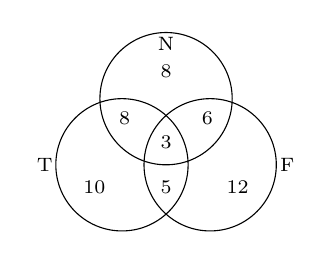
\begin{tikzpicture}[scale=0.7,font=\scriptsize]
\draw (0,0.6) circle(1.2) node[above=14pt]{N}; \draw (-0.8,-0.6) circle(1.2); \draw (0.8,-0.6) circle(1.2);
\node at (0,1.1){8}; \node at (-1.3,-1.0){10}; \node at (1.3,-1.0){12};
\node at (-0.75,0.25){8}; \node at (0.75,0.25){6}; \node at (0,-1.0){5}; \node at (0,-0.2){3};
\node at (-2.2,-0.6){T}; \node at (2.2,-0.6){F};
\end{tikzpicture}
\end{center}
(N$\cap$T only $=11-3=8$, N$\cap$F only $=9-3=6$, T$\cap$F only $=8-3=5$.)

%% Q8 opts
\tikz[baseline=-0.5ex,scale=0.28]{\draw (0,0.45) circle(1); \draw (-0.55,-0.45) circle(1); \draw (0.55,-0.45) circle(1);}
\tikz[baseline=-0.5ex,scale=0.28]{\draw (0,0) circle(1.3); \draw (0,0.35) circle(0.5); \draw (0,-0.35) circle(0.5);}
\tikz[baseline=-0.5ex,scale=0.28]{\draw (0,0) circle(0.8); \draw (1.1,0) circle(0.8); \draw (2.2,0) circle(0.8);}
\tikz[baseline=-0.5ex,scale=0.28]{\draw (0,0) circle(1.2); \draw (0,0) circle(0.9); \draw (0.9,0) circle(0.8);}

%% Q8
Tennis fans, cricket players and students can all overlap (a student may play cricket and follow tennis), and none contains another. So we need \textbf{three mutually intersecting circles}, as in diagram (A).

%% Q9
When the parachute opens, air resistance acts upward. The \textbf{net (total) force} on the man is his weight minus the drag, which is \textbf{less than his weight}. It falls to zero only when he reaches terminal velocity.

%% Q10
This is the \textbf{Fibonacci sequence}: each term is the sum of the previous two. $21+34=55$, $34+55=89$, $55+89=144$, $89+144=233$.

%% Q11 fig
\begin{tikzpicture}
\begin{axis}[ybar,width=8cm,height=4.4cm,bar width=16pt,ymin=0,ymax=400,
  symbolic x coords={1995-96,1996-97,1997-98,1998-99,1999-2000},xtick=data,
  nodes near coords,every node near coord/.append style={font=\tiny},tick label style={font=\scriptsize},
  ylabel={\scriptsize Students in Class I},axis x line*=bottom,axis y line*=left]
\addplot[pattern=north east lines,draw=ink] coordinates {(1995-96,150) (1996-97,200) (1997-98,250) (1998-99,300) (1999-2000,350)};
\end{axis}
\end{tikzpicture}

%% Q11 q
Read the following graph and decide which of the following statement is \emph{false}:

%% Q11
Values: 150, 200, 250, 300, 350.
(A) all are divisible by 25, true. (B) $350>2\times150=300$, true. (D) total growth $=350-150=200$, which is not less than 200, true.
(C) $150:200=0.75$ but $200:250=0.8$, so the ratios are \textbf{not equal}. Statement (C) is \textbf{false}.

%% Q12
Growth is constant at $+50$ students per year: $350+50n>1111\Rightarrow n>15.22\Rightarrow n=16$.
Sixteen years after 1999--2000 is 2015--16, i.e.\ \textbf{2016}.

%% Q13 q
A tyre manufacturing company kept a record of the distance covered before a tyre to be replaced. The following table shows the results of 1000 cases:
\begin{center}\small
\begin{tabular}{lc}\toprule Distance (km) & Tyres replaced\\\midrule Less than 400 & 210\\ 400--900 & 325\\ 900--1400 & 385\\ More than 1400 & 80\\\bottomrule\end{tabular}
\end{center}
If you buy a tyre of this company, what is the probability that it will need to be replaced before it has covered 400 km?

%% Q13
Empirical probability $=\dfrac{210}{1000}=\mathbf{0.21}$.

%% Q14
A correlation of $-0.86$ is a \textbf{high negative} correlation: as the intensity of punishment increases, achievement tends to \textbf{decrease}.
\tip{Correlation shows association, not proof of causation, but in exam language this is read as ``more punishment, lower achievement''.}

%% Q15
Comparing the means of \textbf{two independent groups} (method A vs method B), each of 50 students, calls for the \textbf{t-test}.
\why{Chi-square is for frequencies; the F-test (ANOVA) is for three or more groups; regression is for prediction.}

%% Q16
Per the key, \textbf{bridges} connect two LANs that use the same protocol. (Bridges work at the data-link layer; routers connect different networks.)

%% Q17
Circuit switching (telephone), message switching (store-and-forward) and packet switching (Internet) are all switching techniques: \textbf{each of the three}.

%% Q18
A \textbf{protocol} is a set of rules for communication between \textbf{similar (peer) modules}, i.e.\ the same layer in two systems.

%% Q19
Typical LAN data rates are \textbf{1--100 Mbps} (Ethernet 10/100 Mbps in that period).

%% Q20
Bridges, routers and gateways are all used in wide-area networking: \textbf{each of the three devices}.

%% Q21
Mushrooms are valued as a promising source of \textbf{protein} (with vitamins and minerals), especially for vegetarians.

%% Q22
Nuclear energy comes from both \textbf{fission} (splitting heavy nuclei such as U-235) and \textbf{fusion} (joining light nuclei, as in the Sun).

%% Q23
\textbf{Petroplants} (e.g.\ \emph{Euphorbia}, \emph{Jatropha}) yield latex rich in \textbf{liquid hydrocarbons} that can substitute for petroleum.

%% Q24
Occupational diseases (silicosis, asbestosis, lead poisoning) result from exposure to \textbf{toxic chemicals, dusts and residues} at the workplace.

%% Q25
\textbf{Agricultural waste} (together with firewood and cow dung) is a \textbf{non-commercial} energy source: it is not usually bought and sold. Coal, oil and electricity are commercial.

%% Q26
Educational research has concentrated on children and adolescents and has given relatively little importance to \textbf{adult students' learning styles} (andragogy).

%% Q27
Per the key, linking career advancement to the number of publications \textbf{deteriorates quality}: it encourages quantity over quality (``publish or perish'', predatory journals).

%% Q28
IGNOU offers flexibility in eligibility, age of entry, pace and evaluation. It does \emph{not} prescribe a \textbf{strict combination of courses}; learners may choose.

%% Q29
Spiritual values include non-violence, truth and respect for all religions. \textbf{Untouchability} contradicts them (it is also abolished by Article 17).

%% Q30
The Programme of Action (1992) of NPE 1986 aimed at a mass movement for education, girls' education and pace-setting institutions (Navodaya Vidyalayas). It did not make \textbf{English compulsory for all}.

%% Q31
\textbf{Completing the syllabus in stipulated time} is an administrative target, not an aim of education.

%% Q32
The best way to update teaching competence is to \textbf{experiment with a variety of classroom activities}, i.e.\ reflective practice and learning by doing.

%% Q33
Using an abstraction (rule, principle) in particular, concrete situations is \textbf{application} in Bloom's taxonomy.

%% Q34
A working model is valued for \textbf{showing actions and processes as they develop}, i.e.\ how the thing actually works.

%% Q35
Adolescents' problems are best handled by teachers with \textbf{counselling} skills.

%% Q36
An \textbf{operational definition} states the operations or tasks by which a variable is \textbf{observed and measured} (e.g.\ ``achievement $=$ score on test X'').

%% Q37
In experimental research the researcher \textbf{directly manipulates} the independent variable and \textbf{controls} extraneous variables.

%% Q38
Research must balance freedom and responsibility, so researchers \textbf{follow a code of research ethics} (informed consent, confidentiality, avoidance of harm).

%% Q39
The law of probability applies to \textbf{random sampling}, where each unit has a known, equal chance of selection.

%% Q40
To obtain students' evaluation of teacher performance on various dimensions, a \textbf{rating scale} is the most appropriate tool.

%% Q41 ctx
\textbf{Direction (Q.~Nos.~41 to 45):} Read the following text and answer the questions that follow.\par\smallskip
Human decision-making is being influenced profoundly by modern mathematics, and several particular mathematical subjects have been created primarily to assist in arriving at good decisions. Many aspects involved in arriving at a decision are, of course, nonquantitative in nature. These may relate to history, past experience, instinct, judgement, morality, and so forth. As a consequence, one often refers to decision-making as an art. On the other hand, many ingredients in contemporary decision-making are mathematical in nature, and one can also view this activity as a science.

A decision maker will begin by listing the options over which he or she has some control and the likely outcomes resulting from these choices. The person may attempt to identify all relevant variables and the relationships among them and may associate quantitative measures when possible. Moreover, the decision maker must clarify his or her own values, identify desired goals, and spell out explicitly any limiting resources or social constraints. One then seeks the best possible result obtainable. The situation is typically confounded by a variety of different uncertainties involving data and forecasting that typically cannot be completely resolved in advance. The effect that other decision makers may have on the outcome, and the best responses to their moves, should be predetermined. Various ethical concerns such as fairness may well need consideration, and ways to ascertain group opinions may be necessary. Finally, decision makers must study the social and political context in which the decision will be implemented.

%% Q41 opts
Decision-making is a mathematical activity
Decision-making is a complex intellectual activity
Decision-making is almost impossible
Decision-making is also emotional and social in nature

%% Q41
The passage stresses that besides mathematics, decision-making involves non-quantitative aspects (history, instinct, judgement, morality), group opinion and the social--political context. Per the key, the central idea is that it is \textbf{also emotional and social in nature}.

%% Q42
The situation ``is typically confounded by a variety of different uncertainties involving data and forecasting that typically cannot be completely resolved in advance'', i.e.\ the difficulty of \textbf{exactly predicting the results}.

%% Q43
The decision maker ``may associate quantitative measures \textbf{when possible}'', so using quantitative measures is \textbf{not inevitable}. The other steps are described as necessary.

%% Q44
Decision-making is called an art because many aspects are non-quantitative: history, experience, instinct, judgement, morality, i.e.\ it \textbf{entails personal perspectives}.

%% Q45
Considering ethical concerns such as fairness implies that \textbf{morality is a criterion of a good decision}.

%% Q46
Fast speech with irregular rhythm and long pauses is a paralinguistic sign of \textbf{nervousness} (anxiety).

%% Q47
The \textbf{``You'' attitude} means writing or speaking from the \textbf{receiver's point of view}: their needs, interests and benefits.

%% Q48
A speech that is outlined, practised and delivered conversationally from notes (not memorised or read out) is \textbf{extemporaneous}.
\why{A manuscript speech is read verbatim; an impromptu speech is unprepared.}

%% Q49
To communicate effectively with college students the teacher must \textbf{know the students well}: their background, level, interests and needs.

%% Q50
\textbf{Empathy with the receiver}, i.e.\ understanding the receiver's feelings and viewpoint, leads to the most successful communication.
